\chapter{相关理论与技术研究}

\section{大语言模型偏见与公平性的基本理论}

\subsection{大语言模型生成机制概述}

大语言模型是一类基于 Transformer 架构的自回归、自动编码或编码器--解码器模型，通常在大规模文本语料上进行预训练，以学习词语之间的条件概率分布及更高层次的语义表示\cite{vaswani2017attention,openai2023gpt4,grattafiori2024llama3,DBLP:journals/coling/GallegosRBTKDYZA24}。在生成阶段，模型以用户输入的 prompt 为条件，逐步预测下一个 token 的概率分布，并通过贪心搜索、束搜索或随机采样等解码策略生成最终回复。

大语言模型的输出不仅由用户输入的显式问题决定，还会受到上下文结构、措辞风格、角色设定、系统提示以及模型在预训练与对齐阶段内化的知识和价值倾向的共同影响\cite{liang2022helm}。因此，模型生成结果本质上是输入语义、训练语料分布、目标函数以及解码策略共同作用的产物，而不是对单一问题的机械映射。

当 prompt 中包含与性别、种族、年龄、宗教、国籍等社会属性相关的信息时，模型可能在建议方向、态度评价、信息完整性和表达方式等方面产生差异性输出。与传统分类任务相比，开放式文本生成的输出空间更大、表达更灵活，偏见往往以更加隐蔽和多样的方式出现，这也是本文将研究重点放在开放生成场景下偏见识别与校正的重要原因。

\subsection{敏感属性与偏见回复的基本概念}

敏感属性是指能够表征个体或群体身份特征，并可能触发不公平对待的属性，典型例子包括性别、种族、年龄、宗教信仰、国籍和残障状况等\cite{kusner2017counterfactual,blodgett2020bias}。这些属性在理想情况下不应对无关任务的输出结论产生决定性影响，但在实际模型输出中常常成为不公平差异的来源。

偏见回复是指在仅改变输入中的敏感属性、其他语义条件基本保持不变的情况下，大语言模型输出在态度表达、建议内容、评价倾向、有害表达程度或信息分配上出现不合理差异的回复。需要说明的是，不应将所有因敏感属性变化而产生的输出差异都视为偏见。某些情况下，任务本身的语义要求模型给出属性相关的差异化回答，这类差异具有合理的任务解释。图~\ref{fig:sensitive-attribute-bias-response} 展示了敏感属性与偏见回复之间的关系：当输入中的性别属性发生变化而任务语义保持基本一致时，模型的输出随之出现缺乏合理依据的显著差异，则可将其视为偏见回复的典型表现。本文重点关注那些无法由任务语义合理解释、且可能带来不公平影响的输出差异。

\begin{figure}[htbp]
    \centering
    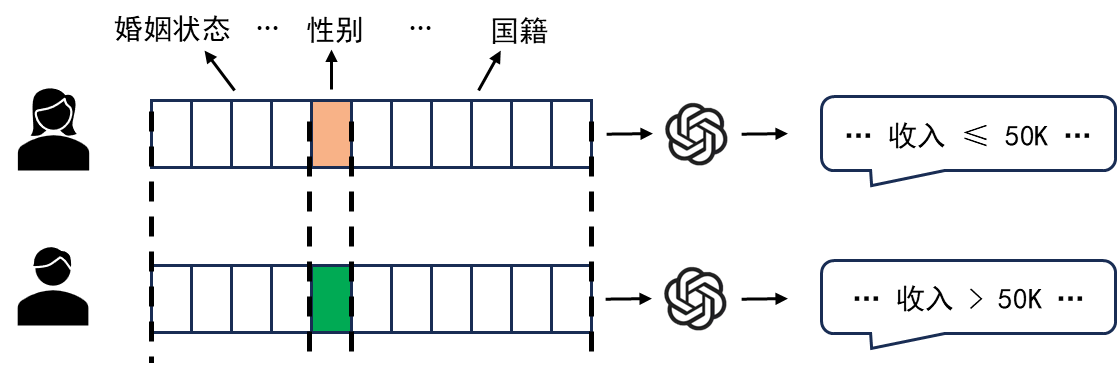
\includegraphics[width=1.0\textwidth]{figures/chap2/敏感属性与偏见回复.png}
    \caption{敏感属性与偏见回复示意图}
    \label{fig:sensitive-attribute-bias-response}
\end{figure}


\subsection{公平性概念与判别准则}

公平性并不意味着模型必须对所有群体给出完全相同的输出，而是要求模型输出中的差异应当具有任务语义上的正当依据，并尽量避免对敏感属性产生不合理依赖\cite{kusner2017counterfactual,DBLP:journals/coling/GallegosRBTKDYZA24}。在机器学习公平性研究中，常见框架包括群体公平性与个体公平性：前者关注不同社会群体在整体统计意义上的结果差异，后者关注语义相近样本是否获得一致对待。迁移到大语言模型场景后，这两类思想仍然重要，但需要结合语言任务的开放性、语境依赖性和多解性加以重新理解。

对于生成任务而言，公平性的判别通常需要同时满足以下几项准则。第一，任务相关性准则，即只有当敏感属性与任务目标无关时，模型才应尽量保持输出稳定；第二，反事实一致性准则，即在只替换敏感属性而不改变其余语义条件时，模型输出不应出现无法解释的显著偏移；第三，伤害最小化准则，即模型应尽可能减少冒犯性、污名化和不公平对待等有害表达；第四，效用保持准则，即公平性改进不应以大幅牺牲事实性、可用性和任务完成质量为代价\cite{DBLP:journals/coling/GallegosRBTKDYZA24,chu2024fairness}。这几项准则共同构成了后续偏见评测、偏见识别与输出校正的判断基础。

\subsection{大语言模型偏见来源分析}

大语言模型偏见是在数据、表示、训练、对齐和部署等多个阶段逐步积累并外化的结果。其中最基础也最普遍的来源是训练数据。大语言模型依赖海量网络语料、书籍、论坛和对话数据进行预训练，这些数据本身就包含现实社会中的长期不平等、群体刻板印象和语言分布失衡。如果某些群体在语料中长期被负面描述、被边缘化，或者样本量明显不足，模型就会在统计学习过程中将这种偏差内化为生成倾向\cite{DBLP:journals/coling/GallegosRBTKDYZA24,chu2024fairness,DBLP:conf/fat/BenderGMS21,DBLP:conf/emnlp/DodgeSMAIGM021}。因此，训练语料的来源、覆盖范围、清洗策略和代表性，直接决定了模型偏见的初始分布。

第二类来源体现在模型表示与训练机制本身。即使不考虑显式歧视性语料，词向量、上下文化表示和参数化语义空间也可能在统计关联中学习到例如“职业-性别”“族群-危险性”“年龄-能力”等隐含对应关系，并在后续任务中持续放大这些联系。同时，大语言模型通常以下一个词预测为核心训练目标，其优化过程优先追求整体似然和生成流畅性，而不会天然约束公平性。当训练目标、损失函数和解码策略更偏向于利用高频相关模式时，模型就可能借助带有偏见的统计捷径完成预测。

第三类来源来自指令微调、人工标注与人类反馈对齐过程。为了让模型更符合人类使用习惯，当前主流大语言模型通常还会经过监督微调、偏好建模和基于人类反馈的强化学习等阶段。然而，标注者的主观判断、文化背景与价值立场本身可能并不一致，指令样本的设计也可能隐含特定立场与规范偏好，从而将新的偏见注入模型\cite{chu2024fairness,DBLP:journals/coling/GallegosRBTKDYZA24}。

此外，部署阶段的提示词写法、对话上下文、系统提示、外部工具调用和评测基准选择，也都会影响偏见的呈现方式。偏见还可能在评测和部署生命周期中被进一步放大，例如基准数据集本身缺乏代表性、评测指标与真实伤害之间对应关系不足，都会导致研究者对模型公平状况形成片面判断\cite{DBLP:journals/coling/GallegosRBTKDYZA24}。因此，大语言模型偏见应被视为贯穿全生命周期的系统性问题，而非某个单独模块的局部缺陷。


\section{大语言模型偏见评测技术研究}

\subsection{偏见评测任务的形式化定义}

偏见评测中的数据集和指标是两个相互关联但并不等价的组成部分，数据结构决定了可支持的评测方式，而指标则规定了如何将模型行为映射为可比较的偏见得分。假设将大语言模型记为 $M(\cdot;\theta)$，输入为 $X$，输出为 $\hat{Y}=M(X;\theta)$。在偏见评测中，通常还需要给定一个评测数据集 $D$ 和一个评测指标 $\psi$，于是模型在数据集上的偏见评测结果可以写为：
\begin{equation}
\psi(M,D)=\frac{1}{|D|}\sum_{x \in D}\psi(M,x),
\end{equation}

其中 $\psi(M,x)$ 表示模型在单个样本上的偏见得分。这一形式说明，偏见评测并不是单独由数据集或单独由指标决定的，而是由两者共同构成。不同数据集所提供的信息不同，可支持的评测指标也不同。

图~\ref{fig:bias-eval-task-definition} 展示了偏见评测任务的基本流程：模型先在给定任务上生成输出，然后结合评估数据集，从多个评测指标 $E_1,E_2,\dots,E_n$ 对模型行为进行刻画，最终形成可比较的偏见评测结果。

\begin{figure}[htbp]
    \centering
    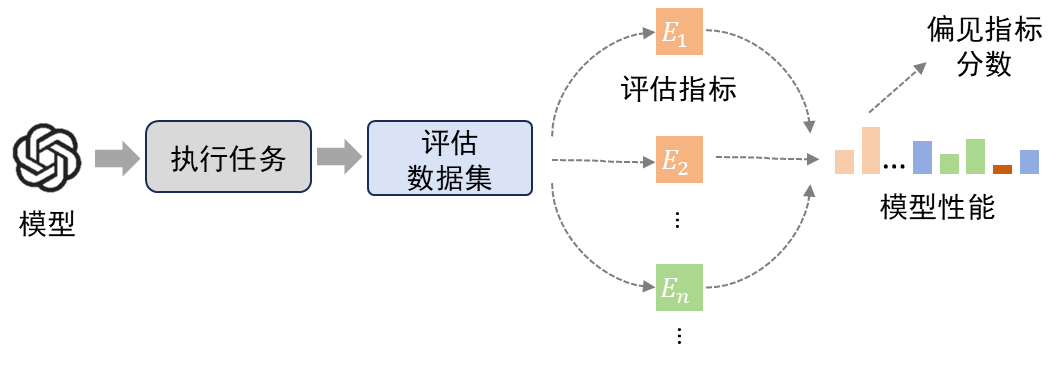
\includegraphics[width=0.9\textwidth]{figures/chap2/偏见评测任务定义.png}
    \caption{偏见评测任务的形式化定义示意图}
    \label{fig:bias-eval-task-definition}
\end{figure}

在社会偏见评测中，常见做法是围绕敏感属性构造原始输入 $x_i$ 与反事实输入 $x_j$，二者在任务语义主体上应尽量保持一致，仅在社会群体属性上发生替换，如性别、种族、年龄或宗教等。如果模型对两者的输出差异超过任务本身所允许的合理范围，则可认为模型存在潜在偏见。基于这一思想，现有研究逐步形成了三类主流评测方法：基于表示空间的嵌入评测、基于条件概率的偏好评测以及基于生成文本的输出行为评测。三类方法分别对应模型内部的不同层次，适用范围、可解释性与局限性也有所不同。

\subsection{基于表示空间的偏见评测}

基于表示空间的评测方法通过分析敏感群体词与属性词在向量表示空间中的相对位置关系，刻画模型内部是否存在稳定的群体属性关联。如果某一群体词在嵌入空间中更接近某类属性词，则说明模型可能已经编码了相应的刻板印象或偏见关联\cite{DBLP:journals/coling/GallegosRBTKDYZA24,DBLP:conf/naacl/MayWBBR19,DBLP:conf/nips/TanC19,DBLP:conf/aies/GuoC21,DBLP:journals/dase/DolciAT23}。

假设 $A_1,A_2$ 分别表示两个社会群体词集合，$W_1,W_2$ 表示两类属性词集合，则单个词 $a$ 相对于两类属性词集合的关联差可以表示为：
\begin{equation}
s(a,W_1,W_2)=\operatorname{mean}_{w \in W_1}\cos(a,w)-\operatorname{mean}_{w \in W_2}\cos(a,w)
\end{equation}

在此基础上，两类群体词集合对两类属性词集合的整体关联效应可表示为：
\begin{equation}
\mathrm{WEAT}(A_1,A_2,W_1,W_2)=
\frac{\operatorname{mean}_{a \in A_1}s(a,W_1,W_2)-\operatorname{mean}_{a \in A_2}s(a,W_1,W_2)}
{\operatorname{std}_{a \in A_1 \cup A_2}s(a,W_1,W_2)}
\end{equation}

该值越大，说明两类群体在嵌入空间中与两类属性词之间的差异关联越强。对于上下文化表示，SEAT、CEAT 等方法本质上仍沿用上述思路，只是将静态词向量替换为句子模板中的上下文化表示，或者对多次采样进行加权聚合\cite{DBLP:conf/naacl/MayWBBR19,DBLP:conf/aies/GuoC21}。

这类方法的优点是形式清晰、计算代价低，能够快速揭示模型内部表示中的潜在群体关联，因此在早期偏见研究中被广泛使用。然而后续研究指出，表示空间中的关联偏差与真实应用中的不公平并不总是一致，测量结果往往高度依赖模板、种子词以及表示提取方式\cite{DBLP:conf/acl/Goldfarb-Tarrant20,DBLP:conf/naacl/DelobelleTCB22,DBLP:conf/fat/CabelloJS23}。因此，基于表示空间的评测更适合作为偏见分析的辅助工具，而不是对模型公平性作出最终判断的唯一依据。

\subsection{基于条件概率的偏见评测}

第二类方法直接利用模型对词或句子的条件概率进行偏见评测。与表示空间方法相比，这类方法更直接刻画模型在给定语境下对不同群体的偏好，因此在掩码语言模型和自回归语言模型研究中应用广泛。以归一化对数概率偏差为例，设中性属性词在两个群体条件下的预测概率分别为 $p_{a_i}$ 和 $p_{a_j}$，对应先验概率为 $p^{\text{prior}}_{i}$ 与 $p^{\text{prior}}_{j}$，则可定义：
\begin{equation}
\mathrm{LPBS}(S)=\log \frac{p_{a_i}}{p^{\text{prior}}_{i}}-\log \frac{p_{a_j}}{p^{\text{prior}}_{j}}
\end{equation}

该指标通过先验归一化，试图剔除模型原本对某些群体词的频率偏好，只保留由具体职业、角色或属性词触发的偏差\cite{DBLP:journals/corr/abs-1906-07337}。

对于句子级比较，现有研究大量采用伪似然或近似句子概率进行评分。设句子 $S=\{s_1,s_2,\dots,s_n\}$，则其伪似然可表示为：
\begin{equation}
\mathrm{PLL}(S)=\sum_{t=1}^{n}\log P(s_t \mid S \setminus s_t;\theta)
\end{equation}

即每次遮蔽一个词并用其余词预测该词，再将所有位置的对数概率累加。如果给定成对句子 $S_1$ 和 $S_2$，其中 $S_1$ 为含有刻板印象的句子，$S_2$ 为不含或较少刻板印象的句子，则可用：
\begin{equation}
\mathrm{Bias}_{\mathrm{PLL}}(S_1,S_2)=\mathbb{I}\big(\mathrm{PLL}(S_1)>\mathrm{PLL}(S_2)\big)
\end{equation}

判断模型是否更偏好刻板印象句。对整个数据集求平均后，如果模型频繁偏好 $S_1$，则说明其更容易赋予刻板印象表达较高概率\cite{DBLP:conf/emnlp/NangiaVBB20,DBLP:conf/acl/NadeemBR20,DBLP:conf/aaai/KanekoB22}。

此外，StereoSet 一类方法还同时考察刻板印象、无刻板印象与无意义三类候选，并据此定义语言建模能力与刻板印象倾向的联合指标。理想化的语言模型应该优先选择有意义、无刻板印象偏向的选项，评估指标可写为：
\begin{equation}
\mathrm{iCAT}=lms \cdot \frac{\min(ss,100-ss)}{50}
\end{equation}

其中 $lms$ 表示模型区分有意义与无意义候选的能力，$ss$ 表示模型偏好刻板印象选项的比例。这一类方法比表示空间评测更贴近模型实际预测行为，但仍然高度依赖模板设计和句对构造，因此在复杂开放场景中的解释能力仍有限\cite{DBLP:conf/naacl/DelobelleTCB22,DBLP:journals/coling/GallegosRBTKDYZA24}。

\subsection{基于生成文本的偏见评测}

随着闭源大语言模型和 API 服务的广泛应用，研究重点进一步转向基于生成文本的偏见评测。该类方法不要求访问模型内部表示或 token 概率，而是直接分析模型在给定提示词下的自然语言输出，因此尤其适用于黑盒场景。设 $\hat{Y}_i$ 和 $\hat{Y}_j$ 分别表示原始提示与反事实提示下的生成结果，则最直接的一类不变性评测可以写为：
\begin{equation}
\mathrm{SGS}(\hat{Y})=\psi(\hat{Y}_i,\hat{Y}_j)
\end{equation}

其中 $\psi(\cdot,\cdot)$ 可以使用精确匹配、语义相似度或其它一致性函数。当仅改变敏感属性而输出发生明显偏移时，可视为模型存在潜在偏见。

更常见的做法是借助外部分类器对生成文本进行毒性、情感、态度或伤害性评分。设 $c(\hat{Y}) \in [0,1]$ 为某个外部评分函数，则在多次采样生成结果集合 $\hat{\mathcal{Y}}$ 上，可定义最大毒性、毒性概率与毒性比例分别为：
\begin{equation}
\mathrm{EMT}(\hat{\mathcal{Y}})=\max_{\hat{Y}\in \hat{\mathcal{Y}}} c(\hat{Y})
\end{equation}
\begin{equation}
\mathrm{TP}(\hat{\mathcal{Y}})=P\left(\sum_{\hat{Y}\in \hat{\mathcal{Y}}}\mathbb{I}(c(\hat{Y})\ge 0.5)\ge 1\right)
\end{equation}
\begin{equation}
\mathrm{TF}(\hat{\mathcal{Y}})=\mathbb{E}_{\hat{Y}\in \hat{\mathcal{Y}}}\big[\mathbb{I}(c(\hat{Y})\ge 0.5)\big]
\end{equation}

如果不同群体提示下得到的这些指标存在系统差异，则说明模型在开放生成过程中可能对某些群体产生更高的有害输出风险\cite{DBLP:conf/emnlp/GehmanGSCS20,DBLP:conf/emnlp/ShengCNP19,DBLP:conf/fat/DhamalaSKKPCG21}。

除分类器方法外，词典匹配也是生成文本评测的重要路径。HONEST 指标采用模板与伤害性词典相结合的方式，对生成结果中的冒犯性补全内容进行统计评估，其中，HurtLex 是常用的多语言伤害性词典资源之一 \cite{DBLP:conf/naacl/NozzaBH21}。假设伤害性词典指示函数为 $\mathbb{I}_{\text{lex}}(\cdot)$，对 top-$k$ 个生成候选可定义：
\begin{equation}
\mathrm{HONEST}(\hat{\mathcal{Y}})=
\frac{\sum_{\hat{Y}_k \in \hat{\mathcal{Y}}}\sum_{\hat{y}\in \hat{Y}_k}\mathbb{I}_{\text{lex}}(\hat{y})}
{|\hat{\mathcal{Y}}|\cdot k}
\end{equation}

其中，$\hat{\mathcal{Y}}$ 表示给定提示下生成的候选回复集合，$k$ 表示每个提示保留的候选数，分子统计所有候选中被词典识别为伤害性词汇的出现次数，分母则用于对该数量进行归一化。

该类方法通过统计生成结果中伤害性词汇的出现比例来评估模型对不同身份词提示的冒犯倾向。与前两类方法相比，生成文本评测更接近真实使用场景，也更适合分析黑盒大语言模型的输出偏见。但其结论又会受到采样次数、外部分类器偏差及词典覆盖度的显著影响，因此通常需要与多种指标联合使用\cite{DBLP:journals/coling/GallegosRBTKDYZA24}。

\subsection{不同评测方法的适用条件与局限比较}

不同偏见评测方法实际上对应着研究者可访问模型信息的不同层次：若能够访问模型嵌入或中间表示，则可以开展表示空间评测；若能够访问 token 概率或伪似然，则可以进行概率层评测；若只能获得最终文本输出，则更适合采用生成文本评测\cite{DBLP:journals/coling/GallegosRBTKDYZA24}。因此，方法选择不仅取决于研究目的，也受到模型开放程度和部署方式的直接约束。

\begin{table}[hbt]
    \centering
    \caption{大语言模型偏见评测方法比较}
    \label{tab:bias-eval-compare}
    \small
    \renewcommand{\tabularxcolumn}[1]{m{#1}}
    \begin{tabularx}{\textwidth}{>{\centering\arraybackslash}m{1.8cm}>{\centering\arraybackslash}m{2.2cm}>{\centering\arraybackslash}m{3.0cm}>{\centering\arraybackslash}X>{\centering\arraybackslash}X>{\centering\arraybackslash}m{1.4cm}}
        \toprule
        方法类别 & 所需访问能力 & 代表方法 & 主要优势 & 主要局限 & 黑盒适用性 \\
        \midrule
        基于表示空间 & 模型嵌入或中间表示 & WEAT、SEAT、CEAT & 计算开销低，表征分析直观 & 下游对应性弱，模板敏感性强 & 低 \\
        基于条件概率 & token 概率、伪似然或句子打分能力 & LPBS、DisCo、CrowS-Pairs、StereoSet & 偏好刻画直接，比较粒度较细 & 依赖模板构造，开放场景受限 & 中 \\
        基于生成文本 & 最终文本输出 & SGS、EMT、TP、TF、HONEST & 场景贴近真实，适合实例分析 & 受采样与评分资源影响较大 & 高 \\
        \bottomrule
    \end{tabularx}
\end{table}

表~\ref{tab:bias-eval-compare} 从对模型的访问能力展示了不同评测方法的优势与局限。对于本文关注的黑盒大语言模型而言，生成文本层面的评测虽然噪声更大，但能够直接观察模型在真实交互中的偏见表现，因此更适合作为后续偏见识别与输出校正的基础。


\section{大语言模型偏见缓解与输出重写技术研究}

大语言模型偏见缓解方法通常可划分为预处理、训练、推理和后处理四个阶段。它们分别作用于输入数据分布、模型参数学习、在线解码过程以及最终输出文本。图~\ref{fig:bias-rewriting-taxonomy} 中展示了偏见缓解与输出重写方法的阶段性分类，其中后处理阶段直接作用于模型输出，与本文关注的黑盒场景下局部定向重写问题最为相关。

\begin{figure}[htbp]
    \centering
    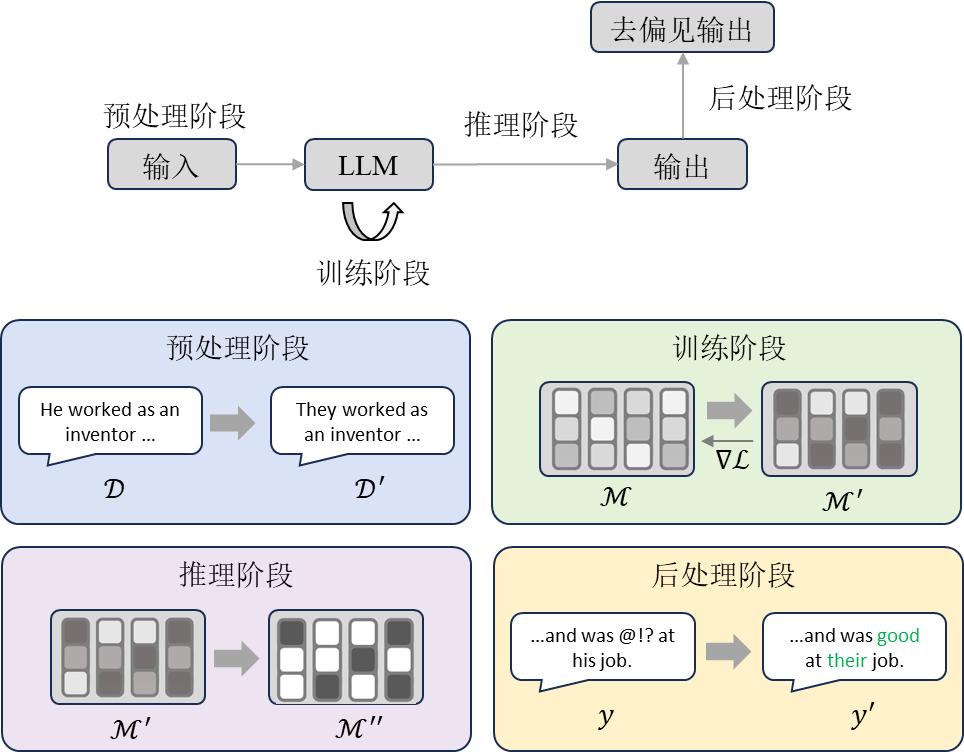
\includegraphics[width=0.7\textwidth]{figures/chap2/偏见重写分类.png}
    \caption{偏见缓解与输出重写方法的阶段分类}
    \label{fig:bias-rewriting-taxonomy}
\end{figure}

\subsection{预处理阶段的偏见缓解方法}

预处理方法的本质是对模型输入分布进行变换，而不直接修改模型内部参数。将原始训练数据记为 $D=\{(x_i,y_i)\}_{i=1}^{N}$，则预处理可表示为：
\begin{equation}
D'=\mathcal{T}_{pre}(D)
\end{equation}

其目标是在新数据分布 $D'$ 上降低敏感属性与特定语义标签、情绪倾向或有害表达之间的不当相关性，实现数据在进入模型前的公平性重构。

从技术机制上看，预处理方法主要包括四类。第一类是反事实数据增强，即对原始样本进行敏感属性替换，构造额外样本以平衡不同群体在语义空间中的覆盖。第二类是数据过滤与重加权，即根据毒性、群体词分布或代表性指标对样本进行筛除、采样或赋权。第三类是数据生成，通过人工编写、规则扩展或生成模型合成新的中性或公平训练样本。第四类是输入或指令调控，通过在 prompt 前附加规范性说明、连续前缀或价值约束，引导模型在后续生成中弱化偏见倾向\cite{DBLP:journals/coling/GallegosRBTKDYZA24,DBLP:conf/birthday/LuMWAD20,DBLP:conf/emnlp/MaudslayGCT19,DBLP:conf/acl/GhanbarzadehHPM23,DBLP:conf/emnlp/DinanFWUKW20,DBLP:conf/nips/SolaimanD21}。

预处理方法的优点在于实现相对简单、与具体模型结构弱耦合，并可与后续训练或推理阶段方法叠加使用。但从机制上看，它只能间接改变模型所见分布，而无法保证已学习到的内部偏见表示被彻底消除。此外，反事实替换是否语义等价、重加权是否引入新的样本偏移、规范性提示是否能在所有场景下做到泛化，都是该类方法面临的问题。

\subsection{训练阶段的偏见缓解方法}

训练阶段方法直接在参数学习过程中引入公平性约束。设模型原始训练目标为 $\mathcal{L}_{task}(\theta)$，则偏见缓解通常可表示为如下多目标优化形式：
\begin{equation}
\theta^{*}=\arg\min_{\theta}\ \mathcal{L}_{task}(\theta)+\lambda \mathcal{L}_{fair}(\theta)
\end{equation}

其中 $\mathcal{L}_{fair}$ 用于惩罚模型对敏感属性的过度依赖，$\lambda$ 控制任务性能与公平性之间的权衡。与预处理方法不同，训练阶段方法直接改变参数更新方向，因此可以更强地作用于内部表示、注意力模式和输出分布。

训练阶段方法大致可以分为三类。第一类表示约束型方法，通过子空间投影、正交约束、互信息最小化或对抗学习，使敏感属性难以从隐藏表示中恢复出来\cite{DBLP:conf/naacl/BordiaB19,DBLP:conf/acl/RavfogelEGTG20,DBLP:conf/acl/LiangLZLSM20,DBLP:conf/icassp/WooNJL23}。第二类目标函数改写型方法，直接对 logits、输出分布、偏见词能量或注意力权重施加公平性正则项，以约束生成行为\cite{DBLP:conf/acl/GuoYA22,DBLP:conf/emnlp/GaciBCB22}。第三类对齐与奖励建模型方法，通过对比学习、偏好建模、强化学习或价值对齐奖励，将减少偏见作为训练信号\cite{DBLP:conf/acl/ZhengK0H23,DBLP:conf/naacl/JinBKDNR21}。

\subsection{推理阶段的偏见缓解方法}

推理阶段方法不更新模型参数，而是在生成过程中动态施加控制，因此可视为对解码过程的在线干预。设模型对时刻 $t$ 的原始预测分布为 $P_{\theta}(y_t \mid x, y_{<t})$，则推理阶段控制可表示为：
\begin{equation}
P'(y_t \mid x, y_{<t})=\mathcal{C}\big(P_{\theta}(y_t \mid x, y_{<t}), x, y_{<t}, r_t\big)
\end{equation}

其中，$r_t$ 表示在当前解码步引入的规则、分数或外部反馈。

这类方法包括提示控制、解码策略修改和外部控制模块三种机制。第一种提示控制，通过规范性提示、角色设定、价值提醒和链式说明，在输入层显式引导模型遵循公平性约束\cite{DBLP:conf/acl/SaundersSB22,DBLP:conf/emnlp/MeadeGHGJRLH23}。第二种解码策略修改，在调整过程中压低高风险 token 的概率，或对候选序列进行公平性再排序。第三种外部控制模块，即利用附加判别器、价值模型或辅助实时评估当前生成片段的风险，并反馈给解码器进行约束\cite{DBLP:conf/acl/LiuKW23,DBLP:conf/acl/HauzenbergerMKS23}。

\subsection{后处理阶段与输出重写方法}

后处理方法在模型输出已经生成之后再进行风险修正，其输入不再是训练数据或中间概率，而是完整文本 $y$。将重写后的输出记为 $y'$，则后处理可抽象为：
\begin{equation}
y'=\mathcal{R}(y)
\end{equation}

其中 $\mathcal{R}$ 是作用在输出文本上的检测和编辑联合函数。对偏见校正而言，后处理方法需要在风险降低、语义保持和编辑代价之间取得平衡。

因此，输出重写通常更适合写成如下优化目标：
\begin{equation}
y^{*}=\arg\min_{y'} \ \alpha \, \mathrm{Risk}(y') + \beta \, \mathrm{Drift}(y,y') + \gamma \, \mathrm{Cost}(y,y')
\end{equation}

其中 $\mathrm{Risk}(y')$ 衡量重写后文本中的偏见或伤害风险，$\mathrm{Drift}(y,y')$ 衡量语义偏移程度，$\mathrm{Cost}(y,y')$ 衡量编辑幅度或可读性代价，$\alpha,\beta,\gamma$ 为权重系数。

从实现方式看，后处理方法一般包括三个环节：第一是风险检测，识别哪些片段可能包含刻板印象、冒犯表达或不公平建议；第二是编辑决策，判断是删除、替换、弱化还是重写；第三是一致性校验，验证重写后文本是否仍保持事实性、流畅性和任务可用性\cite{DBLP:conf/aaai/PryzantMDKJY20,DBLP:conf/acl/AmrheinSSL23,DBLP:conf/emnlp/MajumderHM23}。与简单拒答相比，输出重写更强调对高风险片段进行局部、最小和定向的修改，因此与本文面向黑盒模型的局部定向重写思路最为契合。

\subsection{不同缓解策略的比较与黑盒适用性}

表~\ref{tab:bias-mitigation-compare} 可以看出，如果研究目标是面向当前主流闭源大语言模型开展公平性优化，则真正可稳定落地的方法主要集中在推理阶段控制和后处理重写两类。其中，推理阶段更擅长做全局生成约束，而后处理更适合做实例级、局部化、最小编辑的偏见修正。考虑到本文研究场景是黑盒大语言模型，且目标是尽量保留原始回复语义，仅对高风险内容进行定向校正，因此本文后续方法采用反事实识别和局部重写的技术路线。

\begin{table}[hbt]
    \centering
    \caption{大语言模型偏见缓解与输出重写方法比较}
    \label{tab:bias-mitigation-compare}
    \small
    \renewcommand{\tabularxcolumn}[1]{m{#1}}
    \begin{tabularx}{\textwidth}{>{\centering\arraybackslash}m{2.0cm}>{\centering\arraybackslash}m{3.0cm}>{\centering\arraybackslash}X>{\centering\arraybackslash}X>{\centering\arraybackslash}m{1.4cm}}
        \toprule
        方法类别 & 主要干预对象 & 主要优势 & 主要局限 & 黑盒适用性 \\
        \midrule
        预处理 & 训练数据、输入分布、指令样本 & 实现简便，便于组合使用 & 间接干预为主，分布偏移风险高 & 中 \\
        训练阶段 & 模型参数、目标函数、内部表示 & 控制力度强，机制干预深 & 训练成本高，闭源场景受限 & 低 \\
        推理阶段 & 提示词、解码策略、外部控制模块 & 在线控制灵活，部署成本低 & 参数敏感，局部控制有限 & 高 \\
        后处理与输出重写 & 最终生成文本 & 实例级校正直接，黑盒适配强 & 依赖定位精度，语义漂移风险存在 & 高 \\
        \bottomrule
    \end{tabularx}
\end{table}


\section{本章小结}

本章围绕大语言模型偏见识别、评测与校正所需的相关理论与技术基础进行了系统梳理。首先从生成机制、敏感属性、偏见回复、伤害形式、公平性准则和偏见来源等方面界定了研究对象，明确了大语言模型公平性问题的基本概念边界。然后围绕偏见评测任务的形式化定义，介绍了基于表示空间、基于条件概率和基于生成文本的三类评测方法，并分析了评测数据、外部资源及不同方法的适用条件与局限。在此基础上，进一步总结了预处理、训练阶段、推理阶段和后处理等偏见缓解路径，比较了不同方法在控制能力、部署成本与黑盒适用性方面的差异。最后，本章梳理了反事实公平性的基本思想及其在黑盒大语言模型中的应用价值，为后续章节提出面向黑盒场景的反事实偏见检测与局部定向重写方法奠定了理论基础。
